\documentclass[11pt,a4paper]{article}
\usepackage[margin=25mm]{geometry}
\usepackage[utf8]{inputenc}
\usepackage[T1]{fontenc}
\usepackage{mathpazo}
\usepackage{booktabs}
\usepackage{graphicx}
\usepackage[colorlinks=true,linkcolor=blue,urlcolor=blue]{hyperref}
\usepackage{xcolor}
\usepackage{listings}
\usepackage{setspace}
\usepackage{caption}

\definecolor{titleblue}{RGB}{33,102,172}
\captionsetup{font=small, labelfont=bf}
\onehalfspacing

%% Suppress automatic table/figure numbering — we use manual labels
%% that match the main manuscript's Supplementary Table 1, 2, etc.
\captionsetup[table]{labelformat=empty}
\captionsetup[figure]{labelformat=empty}

\lstset{
  basicstyle=\ttfamily\small,
  breaklines=true,
  frame=single,
  backgroundcolor=\color{gray!5},
}

\begin{document}

\begin{center}
{\LARGE\bfseries\color{titleblue} Supplementary Materials}\\[6pt]
{\large GraphMana: graph-native data management for population genomics projects}\\[4pt]
{\normalsize Jianfeng Mao}
\end{center}

\tableofcontents
\newpage

%% ======================================================================
\section{Supplementary Figure S1: CLI Command Hierarchy}
\label{sec:suppfig1}

\begin{figure}[h]
\centering
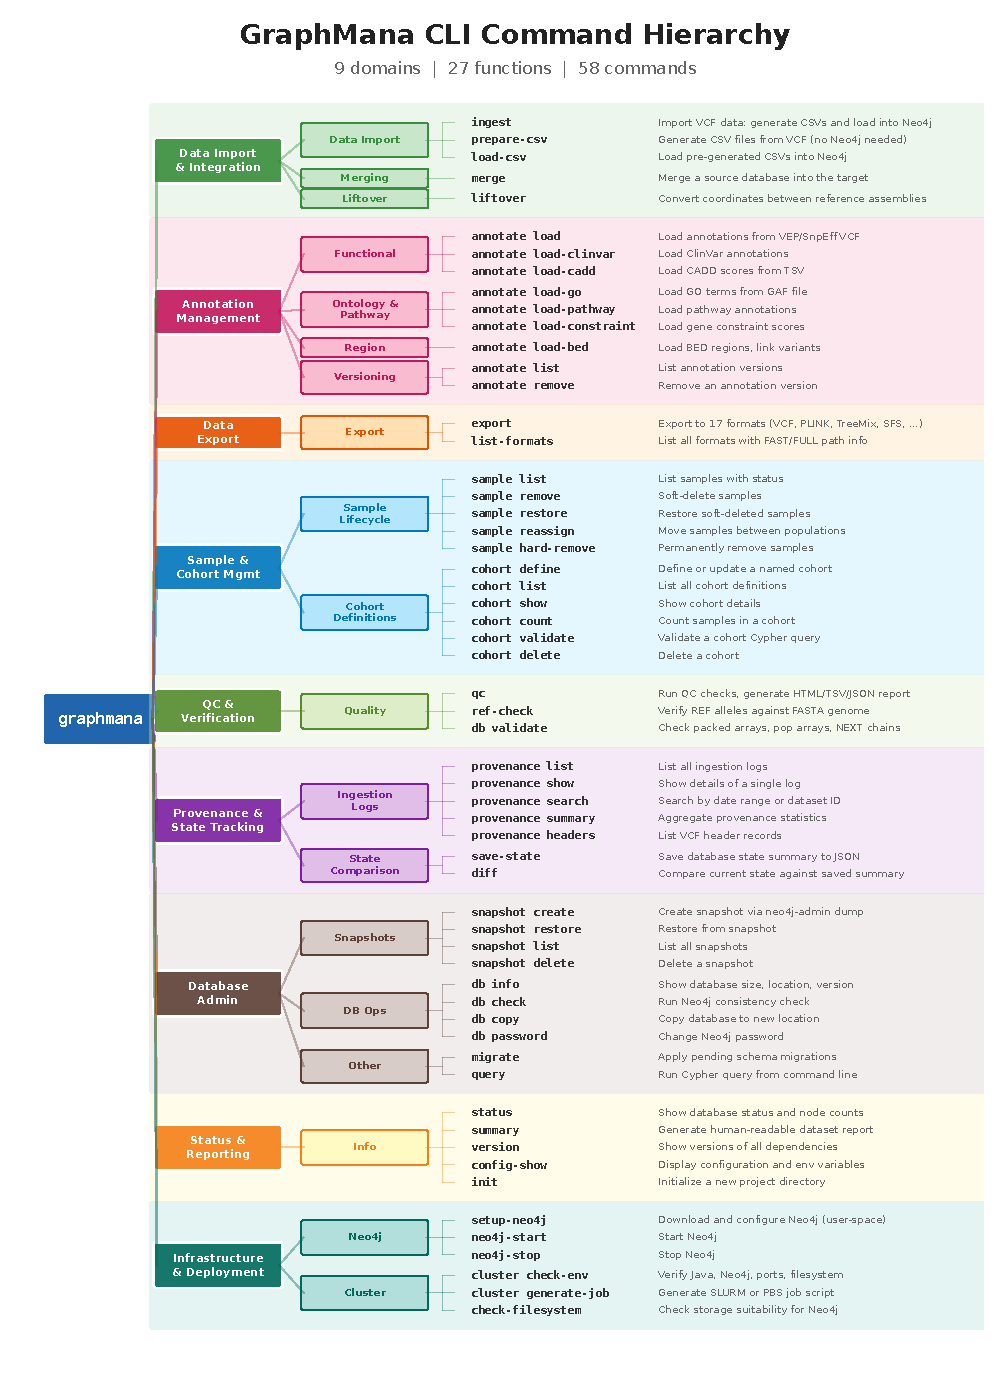
\includegraphics[width=0.85\textwidth]{figures/fig_cli_tree.pdf}
\caption{\textbf{Supplementary Figure 1.} GraphMana CLI command hierarchy. The 58 commands are organized into
9 functional domains and 27 function groups. Each command is accessible as
\texttt{graphmana <command>} with built-in \texttt{-{}-help}.}
\label{fig:cli}
\end{figure}

\newpage

%% ======================================================================
\section{Supplementary Figure S2: Export Manifest Example}
\label{sec:suppfig2}

Each export automatically generates a \texttt{.manifest.json} sidecar file.
Example command:

\begin{lstlisting}[language=bash]
graphmana export --format eigenstrat \
    --populations CEU --populations GBR \
    --populations FIN --populations IBS --populations TSI \
    --chromosomes chr22 --filter-maf-min 0.05 \
    --output european_cohort.eigenstrat
\end{lstlisting}

Resulting manifest (\texttt{european\_cohort.eigenstrat.manifest.json}):

\begin{lstlisting}
{
  "graphmana_version": "1.0.0-dev",
  "timestamp": "2026-03-30T14:22:07.831042+00:00",
  "output_file": "european_cohort.eigenstrat",
  "format": "eigenstrat",
  "n_variants": 439609,
  "n_samples": 633,
  "chromosomes": ["chr22"],
  "filters": {
    "populations": ["CEU", "GBR", "FIN", "IBS", "TSI"],
    "maf_min": 0.05,
    "chromosomes": ["chr22"]
  },
  "recalculate_af": true,
  "threads": 1
}
\end{lstlisting}

The manifest enables any collaborator to verify or reproduce the extraction
without access to the original data manager's notes.

\newpage

%% ======================================================================
\section{Supplementary Table S1: Detailed Benchmark Results}
\label{sec:supptab1}

Chromosome 22, 1.07M variants, 3,202 samples. All timings in seconds.

\begin{table}[h]
\caption{\textbf{Supplementary Table 1a.} Incremental sample addition (3 batches of 234 samples).}
\label{tab:bench1}
\begin{tabular}{@{}lrr@{}}
\toprule
Operation & GraphMana (s) & bcftools (s) \\
\midrule
Initial import / base copy & 602 & --- \\
Batch 1 & 418 & 117 \\
Batch 2 & 412 & 125 \\
Batch 3 & 424 & 133 \\
\textbf{Total} & \textbf{1,856} & \textbf{374} \\
\bottomrule
\end{tabular}
\end{table}

\begin{table}[h]
\caption{\textbf{Supplementary Table 1b.} Cohort-specific VCF extraction (5 superpopulation cohorts).}
\label{tab:bench2}
\begin{tabular}{@{}lrr@{}}
\toprule
Cohort ($N$ samples) & GraphMana (s) & bcftools (s) \\
\midrule
AFR (893) & 191 & 59 \\
EUR (633) & 211 & 51 \\
EAS (585) & 131 & 49 \\
EUR+EAS (1,218) & 238 & 64 \\
ALL (3,202) & 571 & 110 \\
\bottomrule
\end{tabular}
\end{table}

\begin{table}[h]
\caption{\textbf{Supplementary Table 1c.} Multi-format export from a single database.}
\label{tab:bench3}
\begin{tabular}{@{}lrr@{}}
\toprule
Format & GraphMana (s) & bcftools (s) \\
\midrule
VCF & 473 & 96 \\
TreeMix & 189 & N/A \\
SFS (dadi) & 86 & N/A \\
SFS (fsc) & 119 & N/A \\
BED & 84 & N/A \\
TSV & 85 & N/A \\
\bottomrule
\end{tabular}
\end{table}

\noindent\textbf{Annotation update} (53,000 BED regions): GraphMana in-place \textbf{3.5~s},
bcftools VCF rewrite 96~s (\textbf{27$\times$ speedup}).

\noindent\textbf{Lifecycle simulation}: GraphMana 5,880~s (98~min), \textbf{46/46 operations};
bcftools 1,006~s (17~min), 17/26 operations (9 not supported).

\newpage

%% ======================================================================
\section{Supplementary Table S2: Whole-Genome Benchmarks}
\label{sec:supptab2}

70.7M variants, 3,202 samples, 26 populations.

\begin{table}[h]
\caption{\textbf{Supplementary Table 2a.} Whole-genome export timings.}
\label{tab:wg}
\begin{tabular}{@{}llrrr@{}}
\toprule
Format & Path & Variants & Wall time & Size \\
\midrule
TreeMix & FAST & 70,692,015 & 102 min & 780 MB \\
SFS dadi & FAST & 70,692,015 & 98 min & 5.7 KB \\
SFS fsc & FAST & 70,692,015 & 101 min & 1.3 KB \\
BED & FAST & 70,692,007 & 103 min & 2.9 GB \\
TSV & FAST & 70,692,007 & 101 min & 3.8 GB \\
PLINK 1.9 (8 thr) & FULL & 9,627,636 & 156 s & 7.2 GB \\
VCF (BGZF) & FULL & 68,912,619 & 3.7 hr & 14 GB \\
EIGENSTRAT & FULL & 61,599,149 & 3.7 hr & 184 GB \\
\bottomrule
\end{tabular}
\end{table}

\begin{table}[h]
\caption{\textbf{Supplementary Table 2b.} Whole-genome incremental addition (234 samples, CSV-to-CSV rebuild).}
\label{tab:incremental}
\begin{tabular}{@{}lr@{}}
\toprule
Step & Time \\
\midrule
VCF parsing (chr22 batch) & 3 min \\
CSV read + extend + write (214 GB) & 160 min \\
neo4j-admin import & 15 min \\
Database restart + indexes & 4 min \\
\textbf{Total} & \textbf{182 min} \\
\bottomrule
\end{tabular}
\end{table}

\newpage

%% ======================================================================
\section{Supplementary Table S3: Storage and Performance Scaling}
\label{sec:supptab3}

\begin{table}[h]
\caption{\textbf{Supplementary Table 3a.} Storage estimates for whole-genome data ($\sim$85M biallelic variants).}
\label{tab:storage}
\begin{tabular}{@{}lrrrrr@{}}
\toprule
Component & 3,202 & 10K & 50K & 200K & 500K \\
\midrule
gt\_packed & 68 GB & 213 GB & 1.0 TB & 4.3 TB & 10.6 TB \\
phase\_packed & 34 GB & 106 GB & 0.5 TB & 2.1 TB & 5.3 TB \\
Pop arrays & 17 GB & 17 GB & 17 GB & 17 GB & 17 GB \\
\textbf{Total est.} & \textbf{130--200 GB} & \textbf{400--550 GB} & \textbf{2--3 TB} & \textbf{8--10 TB} & \textbf{20--25 TB} \\
\bottomrule
\end{tabular}
\end{table}

\begin{table}[h]
\caption{\textbf{Supplementary Table 3b.} Performance scaling by access path.}
\label{tab:perf}
\begin{tabular}{@{}llrrrr@{}}
\toprule
Operation & Scaling & 3,202 & 10K & 50K & 500K \\
\midrule
FAST PATH & $O(K)$ & Seconds & Seconds & Seconds & Seconds \\
FULL PATH & $O(N)$ & Minutes & Min--hr & Hr--days & Days--wk \\
Incremental & $O(M \times N)$ & 182 min & Hours & Many hr & Days \\
\bottomrule
\end{tabular}
\end{table}

\newpage

%% ======================================================================
\section{Supplementary Table S4: Downstream Tool Compatibility}
\label{sec:supptab4}

Exported from GraphMana 1KGP database (chr22, 3,202 samples, 1,066,557 variants).

\begin{table}[h]
\caption{\textbf{Supplementary Table 4a.} Tier 1: formats validated by loading output into downstream tools.}
\label{tab:compat1}
\begin{tabular}{@{}llllrl@{}}
\toprule
Format & Path & Tool & Variants & Samples & Result \\
\midrule
VCF (BGZF) & FULL & bcftools 1.19 & 1,035,839 & 3,202 & PASS \\
PLINK 1.9 & FULL & PLINK v1.9 & 925,730 & 3,202 & PASS \\
PLINK 1.9 & FULL & PLINK v2.0 & 925,730 & 3,202 & PASS \\
EIGENSTRAT & FULL & convertf v8.0 & 925,730 & 3,202 & PASS \\
TreeMix & FAST & TreeMix v1.13 & 1,066,557 & 26 pops & PASS \\
SFS dadi & FAST & format spec & 1,066,557 & 2 pops & PASS \\
SFS fsc & FAST & format spec & 1,066,557 & 2 pops & PASS \\
\bottomrule
\end{tabular}
\end{table}

\begin{table}[h]
\caption{\textbf{Supplementary Table 4b.} Tier 2: formats verified against published format specifications.}
\label{tab:compat2}
\begin{tabular}{@{}llll@{}}
\toprule
Format & Path & Validation & Result \\
\midrule
BED & FAST & 3+ columns, 0-based & PASS \\
TSV & FAST & Header + columns & PASS \\
JSON Lines & FAST & json.loads per line & PASS \\
Beagle & FULL & Export verified & PASS \\
STRUCTURE & FULL & Export verified & PASS \\
Genepop & FULL & Export verified & PASS \\
\bottomrule
\end{tabular}
\end{table}

\noindent\textbf{Tier 3} (pending external validation): Haplotype, BGEN, GDS, Zarr ---
functional exports that pass internal tests.

\newpage

%% ======================================================================
\section{Supplementary Table S5: Correctness Validation Matrix}
\label{sec:supptab5}

\begin{table}[h]
\caption{\textbf{Supplementary Table 5a.} Variant type import/export correctness.}
\label{tab:correct1}
\begin{tabular}{@{}llllll@{}}
\toprule
Variant Type & Import & Storage & VCF & PLINK & EIGENSTRAT \\
\midrule
Biallelic SNP & PASS & PASS & PASS & PASS & PASS \\
Biallelic indel & PASS & PASS & PASS & excl. & PASS \\
Multi-allelic & PASS & PASS & PASS$^{*}$ & excl. & excl. \\
Structural var. & PASS & PASS & PASS & excl. & excl. \\
Breakend (BND) & PASS & PASS & PASS & excl. & excl. \\
\bottomrule
\multicolumn{6}{l}{\footnotesize $^{*}$Decomposed at import; reconstructed at VCF export.}
\end{tabular}
\end{table}

\begin{table}[h]
\caption{\textbf{Supplementary Table 5b.} Genotype state fidelity and additional dimensions.}
\label{tab:correct2}
\begin{tabular}{@{}llll@{}}
\toprule
Feature & Result & Notes \\
\midrule
HomRef (00) / Het (01) / HomAlt (10) / Missing (11) & PASS & All 4 states roundtripped \\
Phased genotypes & PASS & Per-sample in phase\_packed \\
Haploid samples & PASS & Tracked in ploidy\_packed \\
Annotation add/update/remove & PASS & Genotype layer unaffected \\
Sample order after incremental add & PASS & packed\_index immutable \\
VCF roundtrip (5 samples) & 99.999\%+ & Multi-allelic position ambiguity \\
\bottomrule
\end{tabular}
\end{table}

\noindent 162 tests directly relevant to data correctness, all passing (of 1,439 total).

\newpage

%% ======================================================================
\section{Supplementary Note 1: Export Format Reference}
\label{sec:suppnote1}

17 formats organized by access path. See main text for FAST/FULL PATH definitions.

\noindent\textbf{FAST PATH} (population-level arrays, $O(K)$): TreeMix, SFS-dadi,
SFS-fastsimcoal2, BED, TSV, JSON.

\noindent\textbf{FULL PATH} (per-sample genotypes, $O(N)$): VCF, PLINK~1.9, PLINK~2.0,
EIGENSTRAT, Beagle, STRUCTURE, Genepop, Haplotype, BGEN, GDS, Zarr.

All formats support the full set of export filters.

%% ======================================================================
\section{Supplementary Note 2: Variant Representation}
\label{sec:suppnote2}

Multi-allelic VCF records are decomposed into $K$ biallelic Variant nodes,
each carrying a shared \texttt{multiallelic\_site} identifier and a 1-based
\texttt{allele\_index}. A sample heterozygous for two ALT alleles (VCF
genotype 1/2) is recorded as heterozygous on both nodes. During VCF export,
co-located records are merged back into multi-allelic lines by default.
Structural variants are stored with \texttt{sv\_type}, \texttt{sv\_len}, and
\texttt{sv\_end} properties; genotype calls are encoded identically to SNPs.

%% ======================================================================
\section{Supplementary Note 3: Concrete Workflow Example}
\label{sec:suppnote3}

Five-day workflow demonstrating GraphMana CLI for a typical project.

\subsection*{Day 1: Initial import}
\begin{lstlisting}[language=bash]
graphmana setup-neo4j --install-dir ~/neo4j --memory-auto
graphmana ingest --input data/1kgp_chr*.vcf.gz \
    --population-map data/panel.tsv \
    --neo4j-home ~/neo4j --auto-start-neo4j --threads 16
graphmana status --detailed
\end{lstlisting}

\subsection*{Day 2: Incremental addition (234 new samples)}
\begin{lstlisting}[language=bash]
graphmana save-state --output checkpoints/before_batch2.json
graphmana ingest --input data/batch2.vcf.gz \
    --population-map data/batch2_panel.tsv --mode incremental \
    --neo4j-home ~/neo4j --auto-start-neo4j
graphmana diff --snapshot checkpoints/before_batch2.json
\end{lstlisting}

\subsection*{Day 3: Multi-format export with provenance}
\begin{lstlisting}[language=bash]
graphmana export --format eigenstrat --output exports/european \
    --populations CEU --populations GBR --filter-maf-min 0.05
graphmana export --format treemix --output exports/tree.treemix.gz
graphmana export --format sfs-dadi --output exports/yri_ceu.fs \
    --sfs-populations YRI --sfs-populations CEU \
    --sfs-projection 20 --sfs-projection 20 --sfs-folded
\end{lstlisting}

\subsection*{Day 4: In-place annotation update (3.5 seconds)}
\begin{lstlisting}[language=bash]
graphmana annotate load-clinvar \
    --input annotations/clinvar_20260401.vcf.gz --version ClinVar_2026-04
graphmana db validate
\end{lstlisting}

\subsection*{Day 5: QC and provenance audit}
\begin{lstlisting}[language=bash]
graphmana qc --type all --output reports/qc.html --format html
graphmana ref-check --fasta genomes/GRCh38.fa --chromosomes chr22
graphmana provenance search --since 2026-04-01 --until 2026-04-05
\end{lstlisting}

No file regeneration was required. Each export produced a \texttt{.manifest.json}.
The annotation update did not affect genotype data. The \texttt{diff} command
verified exactly what changed after incremental addition.

\end{document}
